\documentclass[a4paper,11pt]{article}

\input ../include/preamble.tex

\usepackage{tikz}
\usetikzlibrary{automata,arrows,topaths,calc,positioning}

\usepackage{caption}
\usepackage{subcaption}


\begin{document}

\title{
    \textbf{Train shunting}\\
    \large{Programming II - Elixir Version}
}
\author{Christian Schulte \\ \\ {\em adapted to Elixir by Johan Montelius}}
\date{Spring Term 2021}
\maketitle


\thispagestyle{fancy}

\section{Introduction}

You are in charge of shunting wagons of a train.  In
the following we assume that each wagon is self driving and that the
train has no explicit engine.

The description for your shunting task is given by two sequences of
wagons: the given train and the desired train. Your task is to
rearrange the given train with help of your shunting station such that
the desired train is obtained. You are not only supposed to rearrange
the train but also to compute a sequence of shunting moves (which are
called just ``moves'' from now on).


The shunting station is shown in Figure~\ref{fig:station}. It has a
``main'' track and two shunting tracks ``one'' and ``two''.  A
situation in the shunting station is called \emph{state}. A
\emph{move} describes how wagons move from one track to another.

\begin{figure}[h]
\begin{center}
  \begin{tikzpicture}
    \node(main) [rectangle, draw , minimum height=1cm, minimum width=3cm]{main};
    \node(one) [rectangle, draw, minimum height=1cm, minimum width=3cm, above right = 0.5cm and 4cm of main ]{one};
    \node(two) [rectangle, draw, minimum height=1cm, minimum width=3cm, below right = 0.5cm and 4cm of main]{two};
    \draw[<->] (main) to[out=0,in=180](one);
    \draw[<->] (main) to[out=0,in=180](two);    
  \end{tikzpicture}
\end{center}  
\caption{Train shunting station}
\label{fig:station}
\end{figure}

\paragraph{Goal}

Our ultimate goal in this lab is to find a short sequence
of moves that turn a train on the track ``main'' into another
configuration of the train on ``main''.


Before we attempt this goal we will fix the modeling of our
problem and develop some list processing support.

\paragraph{Lab purpose}

This lab exercises several important issues. How are problems modeled
by data structures such as lists and tuples. How are lists
processed. This ranges from simple to more complicated patterns of
recursion over lists. This lab is of course also geared at getting you
started with Erlang and functional programming in general.

And last, but not least, we hope that you have \emph{some fun} solving
this little puzzle.

\section{Modeling}

\paragraph{Trains, wagons, and states}

Wagons are modeled as atoms and trains on tracks as lists of atoms. A
train has no duplicate wagons (that is, \verb+[:a,:b]+ is a train,
whereas \verb+[:a,:a]+ is not).

A complete description of the state of a shunting station
consists of three lists: a list describing the train on track
``main'', and two lists describing tracks ``one'' and ``two''.

\begin{figure}[h]
\begin{center}
  \begin{tikzpicture}
    \node(main) [rectangle, draw , minimum height=1cm, minimum width=3cm]{{\tt [:a, :b]}};
    \node(one) [rectangle, draw, minimum height=1cm, minimum width=3cm, above right = 0.5cm and 4cm of main ]{{\tt [:c, :d] }};
    \node(two) [rectangle, draw, minimum height=1cm, minimum width=3cm, below right = 0.5cm and 4cm of main]{{\tt [:e, :f]}};
    \draw[<->] (main) to[out=0,in=180] (one);
    \draw[<->] (main) to[out=0,in=180](two);    
  \end{tikzpicture}
\end{center}
\caption{Example state displayed.}
\label{fig:ex-state}
\end{figure}

\paragraph{right-most, left-most}

One important question is of course which wagons are the {\em
 right-most} and {\em left-most}. We can of course choose how we
represent our tracks but will chose a way that follows how we write our tracks.

For track one and two the first element in the list will be the wagon
closes to the path to the main track. The first element in the list
that represents the main track is the left-most wagon on the track
i.e. furtests from track one and two.

The state \verb+{[:a,:b],[:c, :d],[:e, :f]}+
is visualized in Figure~\ref{fig:ex-state}.


\paragraph{Moves}

A move is a binary tuple. The first element of a move is either
\verb+:one+ or \verb+:two+. The second element of a move is an
integer. For example, \verb+{:one,2}+, \verb+{:two,2}+, and
\verb+{:one,-3}+ are all moves.

\paragraph{Applying a move to a state}

Moves describe how one state is transformed into another:
\begin{itemize}
\item If the move is \verb+{:one,n}+ and \verb+n+ is greater than
  zero, then the \verb+n+ right-most wagons are moved from track
  ``main'' to track ``one''.

  If there are more than \verb+n+ wagons on track ``:main'', the
  other wagons remain.

\item If the move is \verb+{:one,n}+ and \verb+n+ is less than zero,
  then the \verb+n+ left-most wagons are moved from track ``one''
  to track ``main''.

  If there are more than \verb+n+ wagons on track ``one'', the
  other wagons remain.
\item The move \verb+{:one,0}+ has no effect.
\end{itemize}

The same holds true for moves with first element \verb+:two+
concerning track ``two''.


\begin{figure}[h]
\begin{center}
\begin{tabular}{lr}
  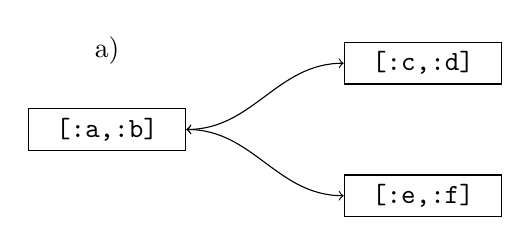
\begin{tikzpicture}
    \node(main) [rectangle, draw , minimum height=0.5cm, minimum width=2cm]{{\tt [:a,:b]}};
    \node(one) [rectangle, draw, minimum height=0.5cm, minimum width=2cm, above right = 0.3cm and 2cm of main ]{{\tt [:c,:d] }};
    \node(two) [rectangle, draw, minimum height=0.5cm, minimum width=2cm, below right = 0.3cm and 2cm of main]{{\tt [:e,:f]}};
    \draw[<->] (main) to[out=0,in=180](one);
    \draw[<->] (main) to[out=0,in=180](two);    
    \node(cap) [rectangle, above of=main] {a)};
  \end{tikzpicture} &
  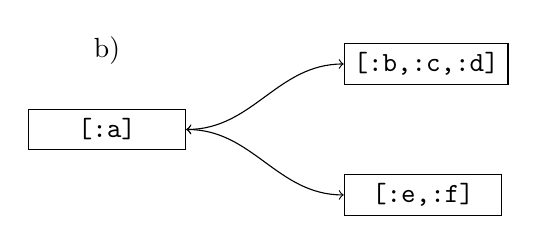
\begin{tikzpicture}
    \node(main) [rectangle, draw , minimum height=0.5cm, minimum width=2cm]{{\tt [:a]}};
    \node(one) [rectangle, draw, minimum height=0.5cm, minimum width=2cm, above right = 0.3cm and 2cm of main ]{{\tt [:b,:c,:d] }};
    \node(two) [rectangle, draw, minimum height=0.5cm, minimum width=2cm, below right = 0.3cm and 2cm of main]{{\tt [:e,:f]}};
    \draw[<->] (main) to[out=0,in=180](one);
    \draw[<->] (main) to[out=0,in=180](two);    
    \node(cap) [rectangle, above of=main] {b)};
  \end{tikzpicture}
  \\[1cm]
  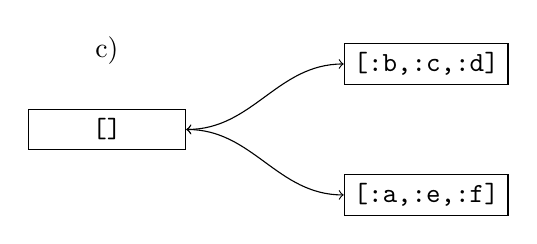
\begin{tikzpicture}
    \node(main) [rectangle, draw , minimum height=0.5cm, minimum width=2cm]{{\tt []}};
    \node(one) [rectangle, draw, minimum height=0.5cm, minimum width=2cm, above right = 0.3cm and 2cm of main ]{{\tt [:b,:c,:d] }};
    \node(two) [rectangle, draw, minimum height=0.5cm, minimum width=2cm, below right = 0.3cm and 2cm of main]{{\tt [:a,:e,:f]}};
    \draw[<->] (main) to[out=0,in=180] (one);
    \draw[<->] (main) to[out=0,in=180](two);    
    \node(cap) [rectangle, above of=main] {c)};
  \end{tikzpicture} &
  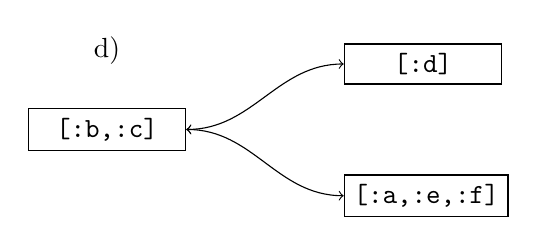
\begin{tikzpicture}
    \node(main) [rectangle, draw , minimum height=0.5cm, minimum width=2cm]{{\tt [:b,:c]}};
    \node(one) [rectangle, draw, minimum height=0.5cm, minimum width=2cm, above right = 0.3cm and 2cm of main ]{{\tt [:d] }};
    \node(two) [rectangle, draw, minimum height=0.5cm, minimum width=2cm, below right = 0.3cm and 2cm of main]{{\tt [:a,:e,:f]}};
    \draw[<->] (main) to[out=0,in=180](one);
    \draw[<->] (main) to[out=0,in=180](two);    
    \node(cap) [rectangle, above of=main] {d)};
  \end{tikzpicture}
\end{tabular}
\end{center}
\caption{Moves applied to states.}
\label{fig:ex-moves}
\end{figure}

\paragraph{Example}

Figure~\ref{fig:ex-moves} shows examples of moves applied to
states, where (a)~is the initial state, (b)~after application of
\verb+{:one,1}+, (c)~after application of \verb+{:two,1}+, and finally
(d)~after application of \verb+{:one,-2}+ (note the order).

\section{Some list processing}

Before we actually start, we will develop some list-processing
routines that you will need later.
\begin{enumerate}

\item \verb+take(xs,n)+ returns the list containing the first \verb+n+
  elements of \verb+xs+.

\item \verb+drop(xs,n)+ returns the list \verb+xs+ without its first
  \verb+n+ elements.

\item \verb+add(xs,ys)+ returns the list where the elements of
  \verb+xs+ have been added to the list \verb+ys+.

  For example, \verb+aff([:a,:b],[:c])+ returns \verb+[:a, :b, :c]+.
  
\item \verb+member(xs,y)+ tests whether \verb+y+ is an element of \verb+xs+.

\item \verb+position(xs,y)+ returns the first position (1 indexed) of \verb+y+ in
  the list \verb+xs+. You can assume that \verb+y+ is an element of
  \verb+xs+.

  For example, \verb+position([:a,:b,:c],:b)+ returns \verb+2+.
\end{enumerate}

Please put all definitions together in one module {\tt Train} in a file \verb+train.ex+


\section{Applying a Single Move}

The first task is writing a binary function \verb+single/2+ that
takes a move and an input state. It returns a
new state computed from the state with the move applied.

For example, \verb+single({:one,1},{[:a,:b],[],[]})+ returns
\verb+{[:a],[:b],[]}+.

\verb+single+ should be used later in this assignment whenever a
move is to be performed on a state.

\paragraph{Structure.}

Now we are in position to develop \verb+single/2+. Approach the
task as follows:
\begin{itemize}
  
\item Your program should decide by pattern-matching which track
  is involved and what the different elements of a state are.
  
\item For a track, you have to decide whether wagons are moved
  \emph{on} or \emph{from} the track (that is, is \verb+n+  positive
  or negative).
  
\item Taking wagons from the end of a train can be done by using
  \verb+length/1+ and \verb+drop/2+; taking wagons from the beginning of a
  train can be done by using \verb+take/2+; adding wagons to a track
  can be done by \verb+append/2+.

\item Take into account that moves are allowed where no wagons
  are moved at all!
\end{itemize}

Please store your function in a module called \verb+Moves+ in the file {\tt moves.ex}.


\section{Shunting}

Develop a procedure \verb+find+ that takes two trains \verb+xs+
and \verb+ys+ as input and returns a list of moves, such that the
moves transform the state \verb+{xs,[],[]}+ into
\verb+{ys,[],[]}+.

In the following, we require that \verb+xs+ and \verb+ys+ contain the
same elements (wagons) and that each wagon is unique (in other
words, \verb+xs+ and \verb+ys+ are permutations of each other).

Approach the problem as follows. The problem is solved
recursively and each recursive step will move one wagon in the
position as required by \verb+ys+.

The base-case is simple. If there are no wagons, no moves are
needed.

Otherwise, we take the last wagon \verb+y+ from \verb+ys+ (the desired
train). Our goal is to find a list of moves that takes the wagon
\verb+y+ from its current position in \verb+xs+ to being the last
wagon in a train on the main track.  This is done by the following
moves:

\begin{enumerate}
  
\item Split the train \verb+xs+ into the wagons \verb+hs+ (for head) and
  \verb+ts+ (for tail), where \verb+hs+ are the wagons before \verb+y+
  in \verb+xs+, and \verb+ts+ are the wagons after \verb+y+ in \verb+xs+.

  Write a procedure \verb+split+ that takes a list of wagons
  \verb+xs+ and the wagon \verb+y+ and returns the pair \verb+{hs,ts}+.

  For example, 
\begin{verbatim}
   split([:a,:b,:c],:a) = {[],[:b,:c]}
   split([:a,:b,:c],:b) = {[:a],[:c]}
\end{verbatim}
  
  Use the functions \verb+position+, \verb+take+, and \verb+drop+.

\item Move \verb\verb+y+ and the following wagons (that is \verb+ts+) on track
  ``one''.
  
\item Move the remaining wagons (that is, \verb+hs+) on track
  ``two''.
  
\item Move all wagons on ``one'' to ``main'' (this includes \verb+y+,
  which goes as needed to the front of ``main'').
  
\item Move all wagons on ``two'' to ``main''.
\end{enumerate}

After having moved one wagon in the right position, we only need
to consider the remaining wagons of both \verb+xs+ and \verb+ys+
(of course in the new order as they are now on the main track!).

Please store your functions in the module \verb+Shunt+ (and file
\verb+shunt.ex+).


\paragraph{Example.}
Given the input train \verb+[:a,:b]+ and the output train \verb+[:b,:a]+, the
list of moves computed by \verb+find+ is:
\begin{verbatim}
   [{:one,1},{:two,1},{:one,-1},{:two,-1} 
    {:one,1},{:two,0},{:one,-1},{:two,0}]
\end{verbatim}




\section{Finding Less Moves}

Develop a function \verb+few+ that behaves as \verb+find+ but
that takes for each recursive application into account whether
the next wagon is already in the right position. If so, no moves
are needed.

Proceed by modifying (only very few modifications are needed)
your program for \verb+find+.

Please store \verb+few+ also in the module \verb+Shunt+.

\paragraph{Example.}
Given the input train \verb+[:c,:a,:b]+ and the output train
\verb+[:c,:b,:a]+, the list of moves computed by \verb+few+ is:
\begin{verbatim}
   [{:one,1},{:two,1},{:one,-1},{:two,-1}]
\end{verbatim}


\section{Move Compression}

The list of moves computed by \verb+few+ is still awkward and
can be easily optimized according to the following rules:
\begin{enumerate}
\item Replace \verb+{:one,n}+ directly followed by \verb+{:one,m}+ with
  \verb-{:one,n+m}-.
\item Replace \verb+{:two,n}+ directly followed by \verb+{:two,m}+ with
  \verb-{:two,n+m}-.
\item Remove \verb+{:one,0}+.
\item Remove \verb+{:two,0}+.
\end{enumerate}

These optimizations are \emph{correct} in the sense that the
shorter list of moves will compute the same final state.

This task is actually tricky: think for example of 
\begin{verbatim}
   [{:two,-1},{:one,1},{:one,-1},{:two,1}]
\end{verbatim}
Repeatedly applying the rules from above actually results in no
moves at all. By application of Rule~1 we obtain
\verb+[{:two,-1},{:one,0},{:two,1}]+;
by Rule~3 
\verb+[{:two,-1},{:two,1}]+;
by Rule~2
\verb+[{:two,0}]+;
and finally by Rule~4
\verb+[]+.

Develop a function \verb+compress+ that takes a list of moves and
returns a compressed list of moves. Compression must be complete,
that is, none of the above rules should be applicable to the
returned list of moves.

Approach this task as follows. Develop a procedure
\verb+rules+ that applies rules recursively. Then repeat
application of \verb+rules+ until the list of moves does not
change. Thus, \verb+compress+ is implemented as follows:
\begin{verbatim}
def compress(ms) do
    ns = rules(ms)
    if ns == Ms do 
       Ms
    else
       compress(ns)
    end
end
\end{verbatim}

Please store your program also in the module \verb+Shunt+.

\section{Finding Really Few Moves}

\emph{This assignment is voluntary.} This means you don't have to
do it, however we strongly encourage you to do it. And actually
it is fun!

The problem with both \verb+find+ and \verb+few+ is that they
always push back the wagons from ``one'' and ``two'' to ``main'',
even though there might be some opportunity to actively use track
``two'' to push wagons from track ``one'' into position and vice
versa. In the following, we are going to take advantage of this.

Develop a procedure \verb+fewer+, that takes four arguments:
\verb+ms+ as the wagons on ``main'', \verb+os+ as the wagons on ``one'',
\verb+ts+ as the wagons on ``two'', and \verb+ys+ as the desired train.

\verb+fewer+ works recursively and as before, each recursive
invocation will bring the first wagon \verb+y+ of \verb+ys+ into the right
position. What is new, is that this wagon might be on either
track:
\begin{itemize}
\item If \verb+y+ is a member of \verb+ms+, bring it in the right
  position as done previously. Leave the other wagons on track
  ``one'' and ``two''.
\item If \verb+y+ is a member of \verb+os+ (it is on track ``one''), move
  the wagons in front first to ``main'' and then to ``two''. Then
  move \verb+y+ into position. Otherwise, leave the wagons on ``one''
  and ``two'' unchanged.

  This adds one more wagon in the right position on ``main''.
\item Do the same for ``two''.
\end{itemize}

Each recursive application of \verb+fewer+ has of course to
supply the wagons on all three tracks correctly!

Initially, \verb+fewer+ is applied such that the tracks ``one''
and ``two'' are the empty list. For example,
\begin{verbatim}
   fewer([:a,:b],[],[],[:b, :a])
\end{verbatim}
returns
\begin{verbatim}
   [{:one,1},{:two,1},{:one,-1},{:two,0},{:one,0},{:two,-1}]
\end{verbatim}

\section{Acknowledgments}

The idea and the initial problem formulation is taken from an
assignment at the 8th Prolog Programming Competition organized by Bart
Demoen and Phuong-Lan Nguyen. 

\end{document}
